\documentclass[a4paper,12pt]{article}

\usepackage{cmap}		
\usepackage[utf8]{inputenc}			
\usepackage[english, russian]{babel}
\usepackage{framed}
\usepackage{hyperref}
\usepackage{amsmath}
\usepackage{graphicx}
\usepackage[colorinlistoftodos]{todonotes}
\usepackage{wrapfig}
\usepackage{lipsum}
\usepackage{listings}
\usepackage{color}
\usepackage{indentfirst}
\usepackage{times}
\usepackage{textcomp}

\definecolor{mygray}{rgb}{0.4,0.4,0.4}
\definecolor{mygreen}{rgb}{0,0.8,0.6}
\definecolor{myorange}{rgb}{1.0,0.4,0}

\lstdefinestyle{customc}{
  belowcaptionskip=1\baselineskip,
  breaklines=true,
  frame=L,
  xleftmargin=\parindent,
  language=C,
  showstringspaces=false,
  basicstyle=\footnotesize\ttfamily,
  keywordstyle=\bfseries\color{green!40!black},
  commentstyle=\itshape\color{purple!40!black},
  identifierstyle=\color{blue},
  stringstyle=\color{orange},
  numbers=left,
  numbersep=12pt,
  numberstyle=\small\color{mygray},
}
\lstset{escapechar=@,style=customc}

\addto\captionsrussian{\def\refname{Список литературы}}
\newcommand{\HRule}{\rule{\linewidth}{0.5mm}}

\begin{document}

\begin{titlepage}
\begin{center}


\includegraphics[width=0.7\textwidth]{pics/logo.png}

\textsc{\normalsize Московский Государственный Университет имени М. В. Ломоносова}\\
\textsc{\small Факультет Вычислительной Математики и Кибернетики}\\
\textsc{\small Кафедра Системного Программирования}\\[1.5cm]

\textsc{\Large Курсовая работа }\\[0.5cm]
\textsc{ \bf \Large  Извлечение логической структуры из сканированных документов }\\[1.2cm]

\vspace{3cm}
\begin{flushright}
Автор: \\
группа 328 \\
Богатенкова Анастасия Олеговна
\end{flushright}
\begin{flushright}
Научный руководитель: \\
Козлов Илья Сергеевич
\end{flushright}

\vspace{3cm}
{ Москва, 2020}\\[0.2cm]

\vfill

\end{center}
\end{titlepage}

\tableofcontents

\newpage 
\section{Введение}

Большое количество текстовой информации представлено в виде pdf-документов, причем эти документы могут 
представлять собой сканированные копии других документов и у них может отсутствовать текстовый слой. При этом размер документов может быть очень большим. Зачастую требуется осуществлять поиск по содержимому таких документов и желательно осуществлять это более эффективным способом.

Как правило, документы имеют логическую структуру и имеют название, разбиение на главы, подглавы и т. д., содержат нумерованные и маркированные списки. Выделение такой логической структуры документа может помочь при решении задач автоматизированного анализа документов, а также при поиске по документам.

Применяется множество разнообразных подходов, которые позволяют выделять в тексте заголовки и распознавать логическую структуру документов.
Для эффективного извлечения такой структуры может быть необходима метаинформация, такая как размер и тип шрифта, отступы, междустрочные интервалы и т. д. 
Поэтому извлечение логической структуры логично делать на этапе анализа сканированных документов.

\newpage
\section{Постановка задачи}

Целью моей курсовой работы является разработка метода выделения логической структуры из документов. Рассмотрим структуру документа в виде глав, подглав (и т. д.), элементов нумерованных и маркированных списков.
Поставим задачу следующим образом: необходимо классифицировать каждую строчку документа как заголовок, элемент списка или текст.

При решении задачи можно выделить следующие этапы ее выполнения:

1) Описание конкретной логической структуры, которую нужно выделить, т. е. разработка манифеста.

2) Разметка корпуса документов для обучения классификатора. Разметка проводится по правилам, указанным в манифесте. 

3) Реализация метода и проведение экспериментальной проверки разработанного метода.

\newpage
\section{Обзор существующих решений}

По извлечению структуры из документов существуют несколько подходов:

- на основе оглавления;

- на основе правил;

- на основе машинного обучения.

\subsection{Извлечение структуры из документов на основе оглавления и правил}

По анализу документов проводится очень много соревнований на ICDAR. В одном из таких соревнований \cite{link1} производилось извлечение структуры из книг, содержимое которых было получено с помощью оптического распознавания символов. Структура книг в виде разбиения на страницы, параграфы, главы извлекалась с использованием оглавления, которое присутствовало в большинстве книг. 

В 2019 году проводились соревнования FinTOC \cite{link2}, где из финансовых документов извлекалась структура в виде иерархии уровней заголовков документов. Максимальная глубина уровней равна пяти. Одна из команд-участниц \cite{link3} извлекала необходимую структуру используя оглавление документов, а также систему правил, которые применялись для определения иерархии заголовков.
Сначала идентифицировались страницы, содержащие текст оглавления, затем в документе находились страницы, соответствующие заголовкам, указанным в оглавлении. 
Последним шагом являлось выделение иерархии найденных заголовков, основанное на применении правил: анализировались такие признаки, как междустрочный интервал, отступ, шрифт, символы нумерации.
Использованный подход позволил получить достаточно высокую точность, но низкую полноту, так как некоторые оглавления документов были неполными.

Извлечение структуры документов на основе оглавления имеет ряд недостатков. Во-первых, невозможно обрабатывать документы, в которых нет оглавления. Во-вторых, при использовании этого метода в структуру документа не будут включаться заголовки, которые не вошли в оглавление, например заголовки более низкого уровня. В-третьих, для нашей задачи необходимо извлекать элементы маркированных и нумерованных списков, которые не включаются в оглавление документа.

\subsection{Извлечение структуры из документов на основе машинного обучения}

В соревнованиях \cite{link2} кроме извлечения иерархической структуры документов решалась задача определения, является ли конкретный блок документа заголовком. Командам был дан набор pdf-документов, xml-файлов с выделенными блоками документов, а так же набор признаков для каждого блока: является ли шрифт блока жирным, курсивом, состоит ли текст из заглавных букв, начинается с заглавной буквы или с нумерации. Кроме данных признаков, каждая из команд использовала различные дополнительные морфологические, семантические, лингвистические признаки. На основе этих признаков обучались различные классификаторы: SVM, MNB, Extra Tree, Decision Tree, Gradient Boosting. Для оценки результатов использовалась F1-мера, максимальный score в соревновании -- 0,982.

Победители соревнования \cite{link5} создали новый датасет для обучения с помощью аугментации данных, перевели новые сгенерированные текстовые блоки в векторное представление, а затем использовали рекуррентные нейронные сети LSTM и BiLSTM для решения задачи классификации. Процесс аугментации показан на схеме ниже.

\begin{center}
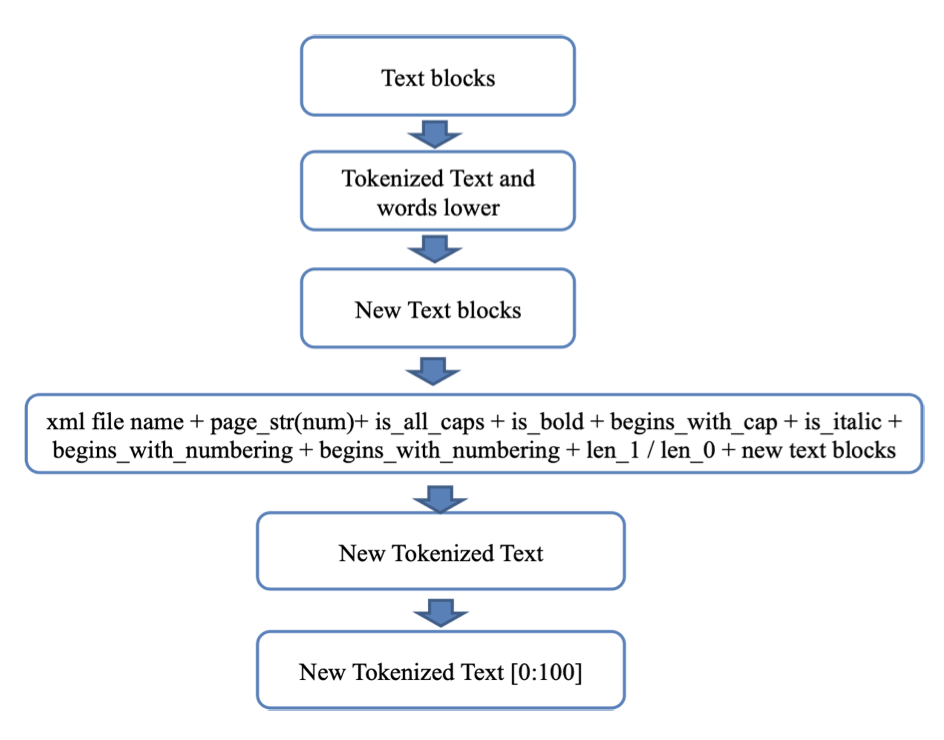
\includegraphics[height=0.5\textwidth]{pics/augmentation.png}
\end{center}

В статье \cite{link4} 2017 года структура документа извлекалась с использованием методов машинного обучения, включая глубокое обучение. Цель данной работы -- автоматически идентифицировать и классифицировать различные секции документов и понять их смысл в рамках документа (назначить семантическую метку). В рамках моей задачи интересна классификация секций документа.

\begin{center}
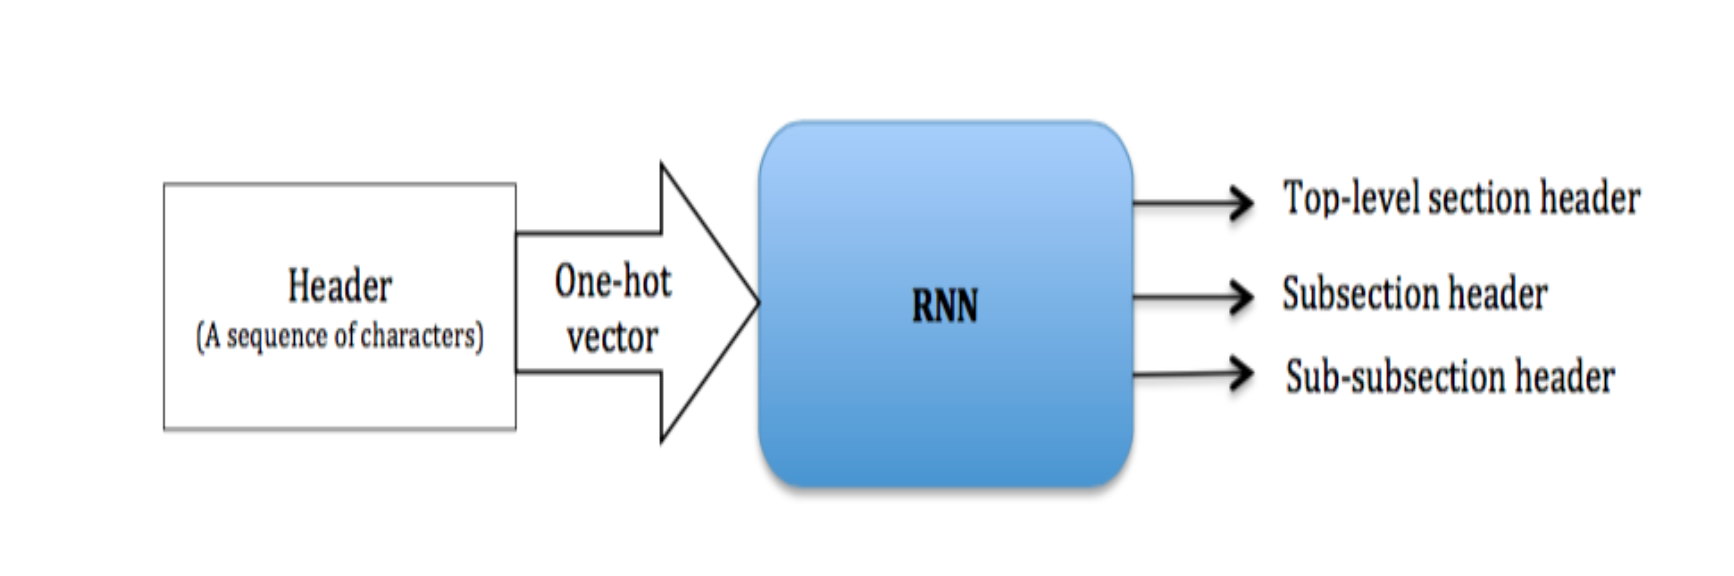
\includegraphics[width=1.0\textwidth]{pics/classifier.png}
\end{center}

Классификатор, который был использован при решении задачи, состоит из нескольких частей. Сначала строки документа подаются на вход классификатору (классификатор строк), который определяет, является ли строка заголовоком, затем строки-заголовки классифицируются точнее другими классификаторами (классификаторы секций). В этом решении структура документа имела вложенность 3, то есть предполагалось выделение секций, подсекций, подподсекций.
Кроме того, в данной работе был размечен датасет, на котором происходило обучение модели. Метрика качества - F1-мера, при идентификации заголовков итоговый score -- 0,96; при классификации секций средний F1-score -- 0,81.

Существующие решения использовать сложно, так как, во-первых, документы, с которыми необходимо работать, могут содержать заголовки или элементы нумерованных списков глубокой вложенности, например 1.1.1.1 (уровней вложенности может быть и больше), а внутри этих уровней могут располагаться нумерованные/маркированные списки, также вложенные.

Во-вторых, как правило в существующих решениях основное внимание уделялось выделению структуры в виде заголовков, для нашей задачи требуется также определять элементы списков.

В-третьих, во большинстве примеров, приведенных выше, осуществляется классификация текстовых блоков, в нашей задаче необходимо классифицировать каждую строку документа.

\newpage
\section{Описание практической части}

\subsection{Описание логической структуры}

Для того, чтобы классифицировать каждую строку документа, необходимо определить, по какому принципу конкретная строка будет относиться к тому или иному классу. Это необходимо при осуществлении разметки корпуса документов для обучения классификатора. 

С этой целью был разработан манифест, прикрепленный в приложении.

\subsection{Подготовка датасета для обучения}

\newpage
\section{Заключение}

\newpage
 
\addcontentsline{toc}{section}{Список литературы}
 \begin{thebibliography}{}
    \bibitem{link1} AntoineDoucet, GabriellaKazai, SebastianColutto, Günter Mühlberger. Icdar 2013 competition on book structure extraction. In Document Analysis and Recognition (ICDAR), 2013 12th International Conference on, pages 1438–1443. IEEE, 2013.
    \bibitem{link2} Rémi Juge, Najah-Imane Bentabet, Sira Ferradans. FinTOC-2019 Shared Task: Finding Title in Text Blocks. 
    \bibitem{link3} Gael Lejeune Emmanuel Giguet. Daniel fintoc-2019 shared task: Toc extraction and title detection. In The Second Workshop on Financial Narrative Processing of NoDalida 2019, 2019.
    \bibitem{link4} Muhammad Mahbubur Rahman, Tim Finin. Deep nderstanding of a Documents Structure. In 4th IEEE/ACM International Conference on Big Data Computing, Applications and Technologies, 2017.
    \bibitem{link5} Ke Tian and Zi Jun Peng. Finance document ex- traction using data augmented and attention. In The Second Workshop on Financial Narrative Process- ing of NoDalida 2019, 2019.
\end{thebibliography}

\newpage
\section{Приложение}

\subsection{Манифест}


Как правило, документы имеют логическую структуру: название, разбиение на главы, подглавы и т. д., нумерованные и маркированные списки. Мы занимаемся извлечением структурных элементов из сканированных документов. Выделение такой логической структуры документа может пригодиться для автоматизированного анализа документов. Мы хотим решать эту задачу как задачу классификации, нам нужно для каждой строки текста определить, к какому типу она относится.

Мы выделяем следующие типы строк: заголовок, элемент списка, текст.

На вход вам будут подаваться документы, в которых выделена прямоугольником одна строка. Вам необходимо для каждой выделенной строки документа определить её тип. Необходимо «Заголовок» пометить цифрой 1, «Список» - 2, «Текст» - 3, «Другое» - 4.

\vspace{1cm}

1) Заголовок

Название главы, секции, подглавы, параграфа. Строка помечается заголовком, если:

-- текст визуально (полностью) выделяется жирностью;

\begin{center}
\frame{
\includegraphics[width=1.0\textwidth]{pics/1.png}}
\end{center}

-- текст полностью выделяется шрифтом (курсив, подчеркнутый, другой шрифт, другой размер шрифта);

\begin{center}
\frame{
\includegraphics[width=1.0\textwidth]{pics/2.png}}
\end{center}

при этом если текст строки выделен шрифтом частично, то заголовком это не считается;

\begin{center}
\frame{
\includegraphics[width=1.0\textwidth]{pics/3.png}}
\end{center}

-- текст выделяется отступом (расположен по центру);

\begin{center}
\frame{
\includegraphics[width=1.0\textwidth]{pics/4.png}}
\end{center}

-- если заголовок занимает несколько строк, остальные строки тоже относятся к типу «заголовок».

\begin{center}
\frame{
\includegraphics[width=1.0\textwidth]{pics/5.png}}
\end{center}

2) Список

Начало нумерованного или маркированного списка. Строка помечается как элемент списка, если:

-- строка наряду с несколькими другими строками пронумерована («1. 1) а) 1.1» и т. д. в начале строки);

\begin{center}
\frame{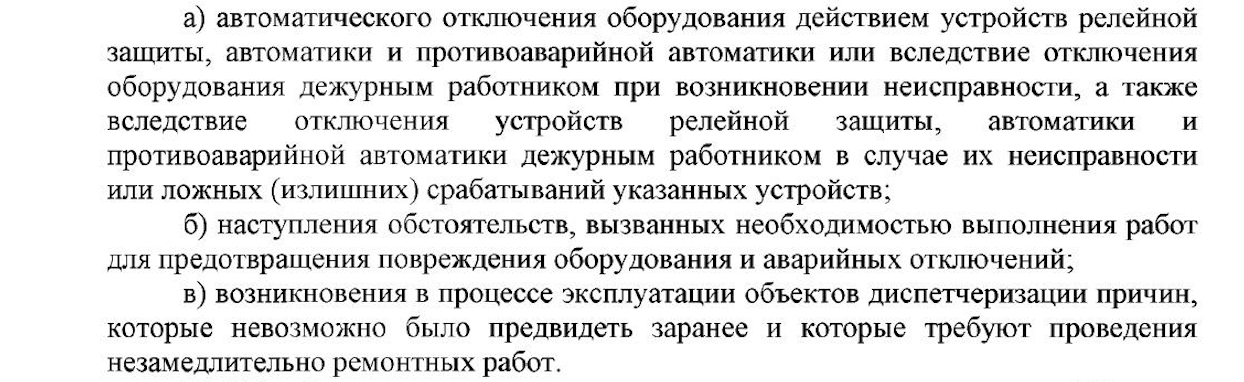
\includegraphics[width=1.0\textwidth]{pics/6.png}}
\end{center}

На картинке выше как элемент списка будут помечены только две строки, остальные помечаются как текст.

\begin{center}
\frame{
\includegraphics[width=1.0\textwidth]{pics/7.png}}
\end{center}

-- строка наряду с несколькими другими выделена некоторым маркером (точка, тире и т. д.) ;

\begin{center}
\frame{
\includegraphics[width=1.0\textwidth]{pics/8.png}}
\end{center}

Здесь как элемент списка будут помечены только две строки, остальные помечаются как текст.


-- если элемент списка визуально занимает несколько строк, все строки кроме первой помечаются как текст. Также к списку не относятся строки, помеченные как заголовок (выделенные шрифтом, жирностью и т. д.).

3) Текст

Все остальные строки, содержащие текст документа, помечаются как текст.

На вход вам будут подаваться документы, в которых выделена прямоугольником одна строка. Вам необходимо для каждой выделенной строки документа определить её тип. Необходимо «Заголовок» пометить цифрой 1, «Список" - 2, «Текст» - 3. В случае, если прямоугольником выделена строка, не содержащая текст (пустая строка, рукописная подпись, печать), строку необходимо пометить как «Другое» (цифра 4), либо пропустить данную строку при разметке.

Ниже приведен пример разметки. Красными прямоугольниками выделены заголовки, зелёными - элементы списков, а синими - текстовые блоки.

\begin{center}
\frame{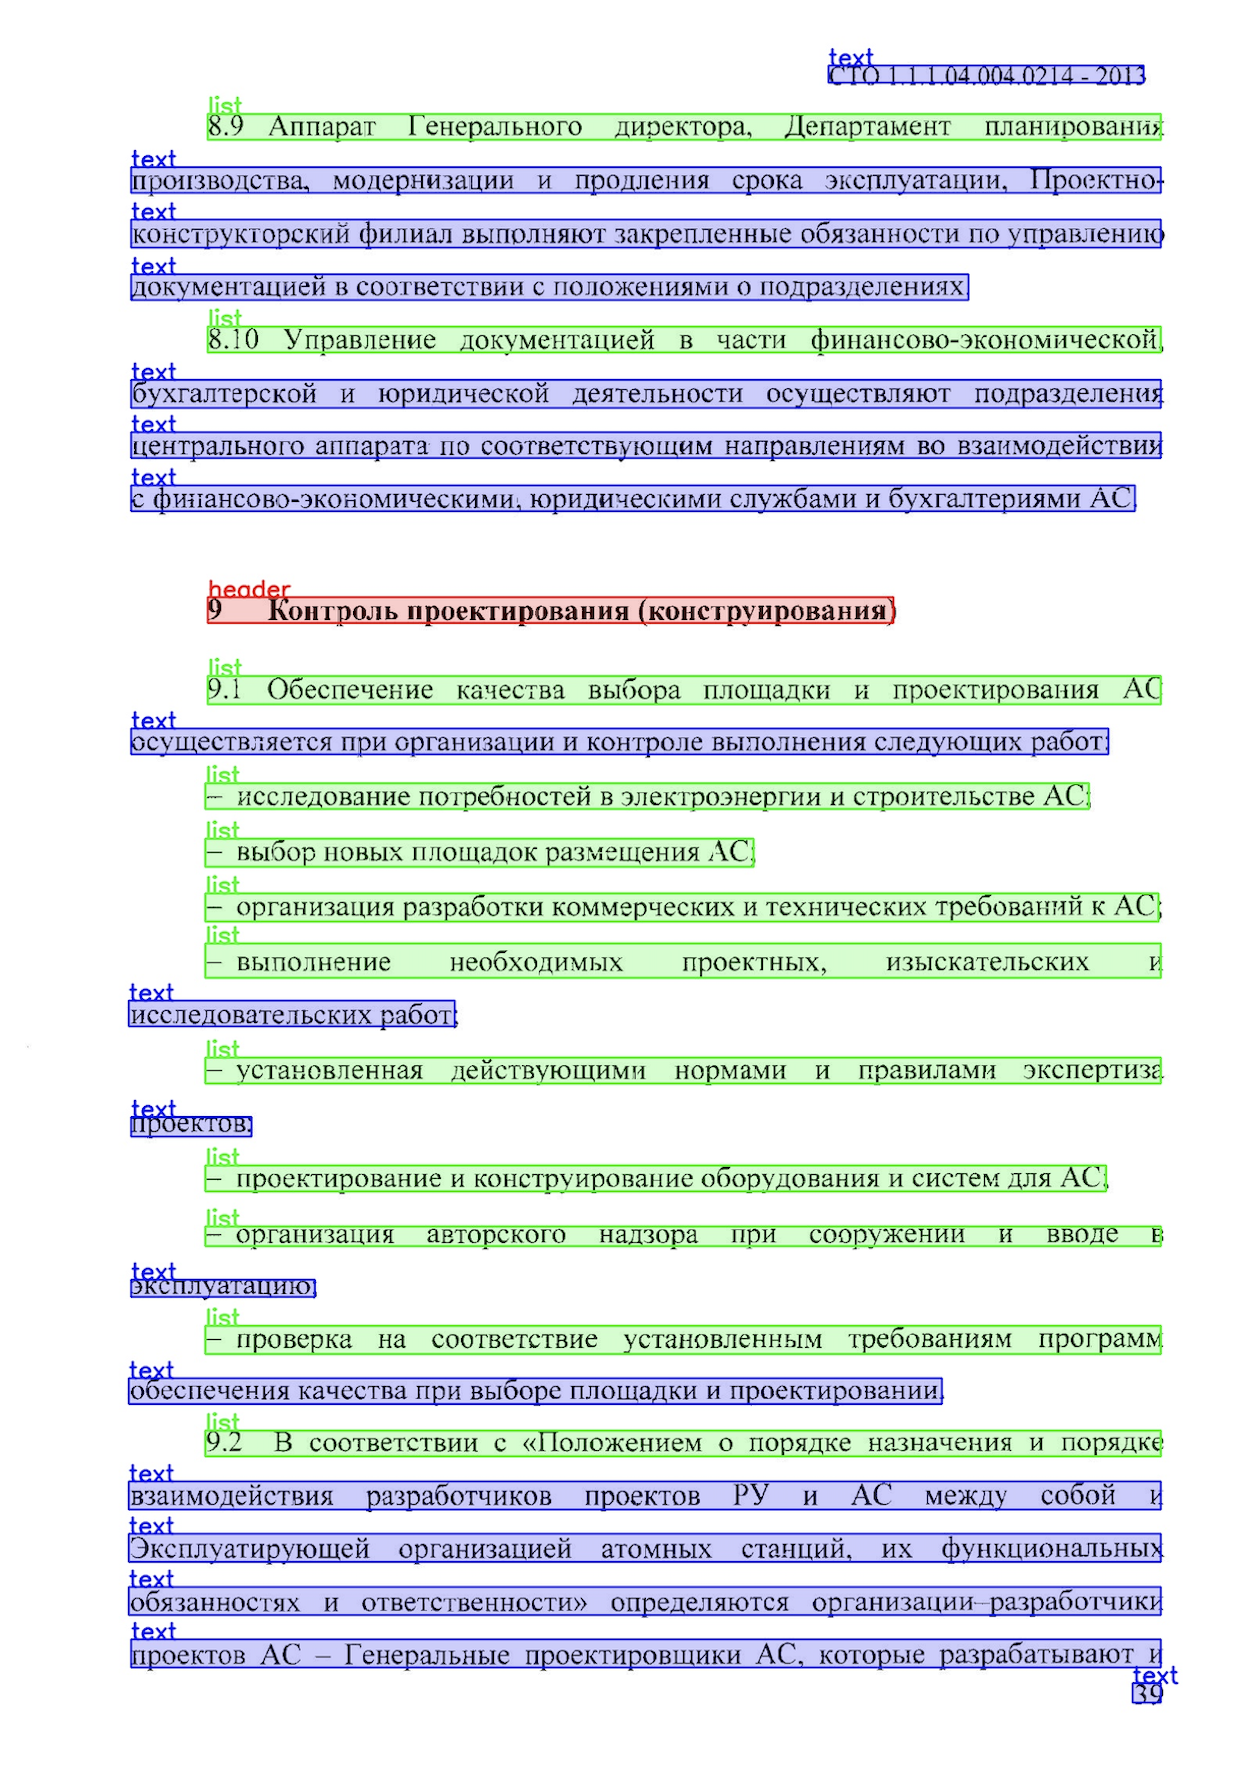
\includegraphics[height=1.0\textwidth]{pics/example.png}}
\end{center}

\end{document}
